\chapter{Materials and Methods}\label{chap:materials-methods}
This chapter introduces the materials and datasets provided in the source paper \citep{Ferber2024}. We then describe how the data were preprocessed and explored, explain how the models were implemented, trained, and evaluated, and finally present the methods used to analyse model explainability.

\section{Data and Materials}\label{sec:method-data-materials}
As part of \citet{Ferber2024}, the authors have published a dataset of 1798 \glspl{subject} running or walking on a treadmill captured using multi-camera 3D \gls{mocapsys}. The dataset is composed of raw 3D~marker data of each \gls{session}, descriptive biomechanical variables derived from the marker data for each session and demographic and anthropometric metadata of the subjects. Additionally, the matlab code for the preprocessing of the data, the calculation of the kinematic variables and tutorial notebooks that help lustrate how to use their library and read the data from the folder structure are also provided. Although both walking and running data is provided, we have used exclusively running data. From this point onwards, walking data is ignored for brevity.

\subsection{Measurement protocol}\label{subsec:measurement-protocol}
The complete measurement protocol is described in \citet{Ferber2024}. In this subsection, we provide a summary of the aspects that are most relevant for the methods and analyses presented in this thesis.

The raw marker data was collected using high-speed optoelectronic infrared-based motion capture cameras (MX3/Bonita, Vicon, Oxford, UK) were used to record the position of 9~mm spherical retro-reflective markers attached to anatomical landmarks of the subjects at either 120~Hz or 200~Hz. Depending on the lab, eight or three cameras were used. Below we list and describe the three sets of markers that were used.
\begin{itemize}
    \item \textbf{Core}: Markers attached to the following anatomical landmarks: medial and lateral malleoli, medial and lateral femoral condyles, and greater trochanters.
    \item \textbf{Additional}: Markers attached to the following anatomical landmarks: bilateral 1st and 5th metatarsal heads, distal aspect of the shoe, tibial tuberosity, anterior superior iliac spines, and iliac crests;
    \item \textbf{Clusters}: 3 or 4 markers placed on rigid shells attached to the following anatomical landmarks: sacrum, bilateral thigh and shank, and posterior aspect of both shoes.
\end{itemize}

During the recording of the sessions of all 1798 subjects the 'core' and 'cluster' set of markers were used. The additional set was only used during the recording of the sessions of 1082 subjects. Figure \ref{fig:marker_position} shows the lower body of a subject and the three sets of markers.

\begin{figure}[ht]
    \begin{centering}
    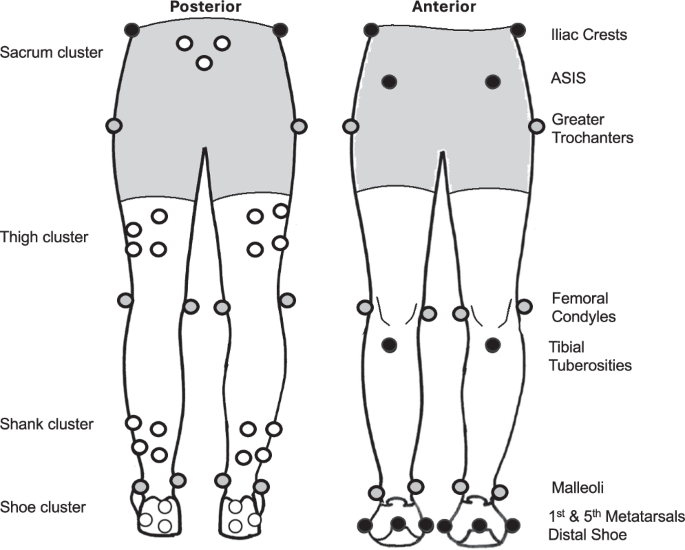
\includegraphics[width=0.5\columnwidth]{images/billateral_marker_position.png}
    \par\end{centering}
    \caption{Position of markers on the subjects. Grey markers correspond to core set of markers set, black to additional set and white to the clusters set. Source: \citet{Ferber2024}}
    \label{fig:marker_position}
\end{figure}

% TODO: Explain the recording procedure: Warm up, duration, discard, etc...

\subsection{Dataset Description}\label{subsec:method-dataset-description}
As described above, the dataset contains two complementary components: (i) session-level metadata stored as tabular files, and (ii) motion-capture marker data together with derived kinematic variables per session. Below we describe each component and list the variables that are available for analysis.

\paragraph{Metadata File (tabular)} The metadata file is provided as a CSV file: \texttt{run\_data\_meta.csv}. Each row corresponds to a single treadmill session recorded for a subject. It contains anthropometric and demographic variables.
\begin{itemize}
    \item \texttt{sub\_id}: Unique subject identifier.
    \item \texttt{datestring}: Session recording date.
    \item \texttt{filename}: Session filename used to locate the marker json file for the session.
    \item \texttt{speed\_r}: Treadmill belt speed (m/s).
    \item \texttt{age}: Subject's age (years).
    \item \texttt{Height}: Body height (cm).
    \item \texttt{Weight}: Body weight (kg).
    \item \texttt{Gender}: Subject gender.
    \item \texttt{DominantLeg}: Dominant leg (Left/Right/Ambidextrous).
    \item \texttt{InjDefn}: Injury severity reported by the subject choosing between 4 options: (1) No Injury, (2) Continuing to train in pain, (3) Training volume/intensity affected, (4) Minimum of two workouts missed in a row.
    \item \texttt{InjJoint}, \texttt{InjSide}, \texttt{SpecInjury}, \texttt{InjDuration}: Primary injured joint, side (Left/Right), Specific injury diagnosis from medical professional, and for how long has the subject had the injury.
    \item \texttt{InjJoint2}, \texttt{InjSide2}, \texttt{SpecInjury2}: Secondary injury information (if applicable).
    \item \texttt{Activities}: Subject reported athletic activities performed on a regular basis.
    \item \texttt{Level}: Self-reported level of athletic activity (recreational/competitive).
    \item \texttt{YrsRunning}: Number of years subject has been running on a regular basis.
    \item \texttt{RaceDistance}: Preferred race distance.
    \item \texttt{RaceTimeHrs}, \texttt{RaceTimeMins}, \texttt{RaceTimeSecs}: Preferred race distance best time.
    \item \texttt{YrPR}: Year of preferred race distance personal best time.
    \item \texttt{NumRaces}: Number of races completed per year.
\end{itemize}

\paragraph{Marker and descriptive biomechanical data (Hierarchical)} For each session, 3D positions of reflective markers and descriptive variables derived from those markers are provided as json files. One file per session.
\begin{itemize}
    \item \textbf{Recording frequency} Frequency of the recording in Hertz (Hz). Either 120 Hz or 200 Hz depending on the lab.
    \item \textbf{Joint Marker Neutral}: 3D coordinates of the individual markers of the core and additional marker sets while the subject is standing in neutral position.
    \item \textbf{Cluster Marker Neutral}: 3D coordinates of the individual markers in the cluster marker set while the subject is standing in neutral position.
    \item \textbf{Dynamic Marker data}: 3D coordinates at each of the frames of the recording for the individual markers in the cluster marker set.
    \item \textbf{Descriptive biomechanical variables}: Set of 77 variables derived from the 3D coordinates Marker data. Calculated for Left and Right side of the body.
\end{itemize}

It must be noted that \texttt{Joints} and \texttt{Neutral} coordinates do not represent the true anatomical centres, only the centres of the markers on the skin of the subject.
Only 33 of the 77 descriptive biomechanical variables are populated per side, the rest all contain 0 for all values of all sessions, this totals 66 populated descriptive variables in total. Table \ref{tab:met-desc-variable-init} describes the variable set per side.

% TODO: Breakdown into one table per group and analyse that group individually....
\begin{table}[ht]
    \centering
    \caption[Populated Descriptive Variables Summary]{Summary of the Descriptive Biomechanical Variables that are populated\label{tab:met-desc-variable-init}}
    \begin{tabular}{lp{0.6\textwidth}}
    \hline
    \textbf{Variable} & \textbf{Category} \\
    \hline
    Step width (m) & Temporal-spatial \\
    Stride rate (steps/min) & Temporal-spatial \\
    Stride length (m) & Temporal-spatial \\
    Swing time & Temporal-spatial \\
    Stance time & Temporal-spatial \\
    Peak drop angle & Pelvis kinematics \\
    Drop excursion & Pelvis kinematics \\
    Dorsiflexion peak angle & Ankle kinematics \\
    Ankle Eversion peak angle & Ankle kinematics \\
    Ankle Rotation peak angle & Ankle kinematics \\
    Ankle Eversion excursion & Ankle kinematics \\
    Ankle Rotation excursion & Ankle kinematics \\
    Ankle Eversion \% of stance & Ankle kinematics \\
    Knee Flexion peak angle & Knee kinematics \\
    Knee Adduction/abduction peak angle & Knee kinematics \\
    Knee Rotation peak angle & Knee kinematics \\
    Knee Adduction/abduction excursion & Knee kinematics \\
    Knee Rotation excursion & Knee kinematics \\
    Hip Extension peak angle & Hip kinematics \\
    Hip Adduction peak angle & Hip kinematics \\
    Hip Rotation peak angle & Hip kinematics \\
    Hip Adduction excursion & Hip kinematics \\
    Hip Rotation excursion & Hip kinematics \\
    Foot progression angle & Foot kinematics \\
    Heel-strike angle & Foot kinematics \\
    Medial heel whip excursion from toe-off & Foot kinematics \\
    Ankle eversion peak velocity & Joint velocities \\
    Ankle rotation peak velocity & Joint velocities \\
    Knee adduction peak velocity & Joint velocities \\
    Knee abduction peak velocity & Joint velocities \\
    Hip abduction peak velocity & Joint velocities \\
    Knee rotation peak velocity & Joint velocities \\
    Hip rotation peak velocity & Joint velocities \\
    Pelvic drop peak velocity & Joint velocities \\
    Pronation onset \% of gait cycle & Foot timing \\
    Pronation offset \% of gait cycle & Foot timing \\
    Vertical oscillation (mm) & Vertical oscillation \\
    \hline
    \end{tabular}
\end{table}

All descriptive variables follow the interpretations described in \citet{Bartlett2014}. Unless specified explicitly in the table, the units are degrees for angles and excursions, and degrees/s for joint velocities. Excursions are also commonly known as range of motion (ROM) in the literature.
% TODO: Explain important biomechanical concepts like dorsiflexion, eversion, etc...

\subsection{Code Description}\label{subsec:method-code-description}
Python was the main language used in this project, although several scripts were implemented in \GLS{matlab} for the data acquisition and extraction stages. Matlab was also used to preprocess the dataset, following the procedure described in the source paper. All code created for this project and used to generate the reported results has been made publicly available for reproducibility \cite{Zapater_Reig_Running_Injury_Clinic_2025}.

The MATLAB reference implementation published with the dataset in \citet{Ferber2024} was employed as part of this work. The corresponding MATLAB scripts have been included in the repository under the \texttt{supplemental\_material} folder for consultation.

The following assets are the most relevant components of the repository:

\paragraph{Notebooks}
\Gls{jupyter} notebooks used during development. These capture the iterative process across the different phases of the project and the reporting of results.

\paragraph{\texttt{core} Package}
Python package containing the core functionality used in the notebooks. It includes classes, functions, and constants to orchestrate data extraction, preprocessing, feature engineering, model training, and evaluation.

\paragraph{\texttt{gait\_kinematics.m}}
Script provided with the source paper. It calculates joint angles and angular velocities from the \texttt{Dynamic Marker Data}, \texttt{Joint Marker Neutral}, and \texttt{Cluster Marker Neutral} files. Anatomical segment coordinate systems are constructed from the neutral marker data, segment motion is tracked using the dynamic marker data, and XYZ Cardan joint angles and angular velocities are computed. The script returns:
\begin{itemize}
    \item \texttt{Angles}: per-frame joint/segment angles for the left/right ankle, knee, hip, as well as foot and pelvis segments (degrees).
    \item \texttt{Velocities}: per-frame angular velocities for the same structures (deg/s).
    \item \texttt{jc}: estimated joint centre positions (pelvis, hips, knees, ankles).
\end{itemize}

\paragraph{\texttt{gait\_steps.m}}
Script also provided with the source paper. It calculates descriptive biomechanical variables from the \texttt{Dynamic Marker Data}, \texttt{Cluster Marker Neutral}, \texttt{Angles}, and \texttt{Velocities}. The script returns:
\begin{itemize}
    \item \texttt{event}: gait cycle events by side (touchdown, mid-stance, toe-off, heel whip).
    \item \texttt{Descriptive biomechanical variables}: as defined in Table~\ref{tab:met-desc-variable-init}.
\end{itemize}

\paragraph{\texttt{processing\_source\_data.m}}
Script implemented for this project to process the metadata file and marker-data JSON files. Joint angles, joint angular velocities and cycle events are computed by calling \texttt{gait\_kinematics.m} and \texttt{gait\_steps.m}. The outputs are converted into tabular format for the exploratory data analysis (EDA) stage.


\subsection{Data Extraction}\label{subsec:data-extraction}

The script \texttt{processing\_source\_data.m} was executed to process the raw dataset. Out of 2506 recorded sessions (with some subjects contributing multiple sessions), 2487 were processed successfully, of which 1813 contained valid running data. Sessions without running data or those where MATLAB preprocessing failed were excluded.

The outputs consist of time-series data for markers, joint angles, joint angular velocities, and detected gait cycle events with their corresponding frame indices. These outputs were further processed using the \texttt{pandas} and \texttt{kinetics-toolkit} Python packages to combine the event information with the time-series data.

Figure \ref{fig:data-ext-marker-velo-angle-ts} illustrates an example from a single session, showing the raw marker data for one marker in the left shank cluster together with the corresponding joint angle and angular velocity for the left knee. Figure \ref{fig:data-ext-l-knee-angle-events} shows frames 500--1000 of the left knee angle, annotated with the touchdown and toe-off events. Figure \ref{fig:data-ext-marker-3d} provides a 3D representation of a frame with the full marker set.

In addition to the time-series data, the script also generates the a of 33 descriptive variables. These variables are equivalent to those stored in the JSON files of the source dataset. To validate the execution of \texttt{processing\_source\_data.m}, the generated variables were compared against the source dataset. All variables matched within a relative tolerance of $1 \times 10^{-9}$, except for 35 values of \texttt{speed\_r}, which differed by $9 \times 10^{-2}$. This deviation is negligible when measuring human running speed in m/s and confirms that the execution was successful. The resulting data was considered ready for the exploratory data analysis stage.

\begin{figure}[ht]
    \centering
    \begin{minipage}[t]{0.48\textwidth}
        \centering
        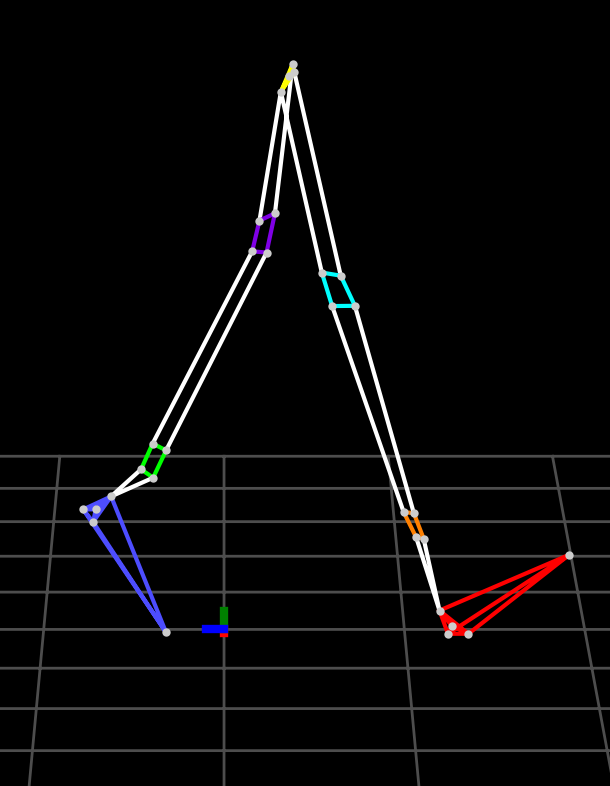
\includegraphics[width=\textwidth]{images/ex_3d_marker.png}
        \caption{3D representation of a frame with all marker data. Connecting lines have been added between markers. The left foot is coloured blue and the right foot red. From top to bottom: pelvis, left/right thigh, left/right shank, and left/right foot.}
        \label{fig:data-ext-marker-3d}
    \end{minipage}
    \hfill
    \begin{minipage}[t]{0.48\textwidth}
        \centering
        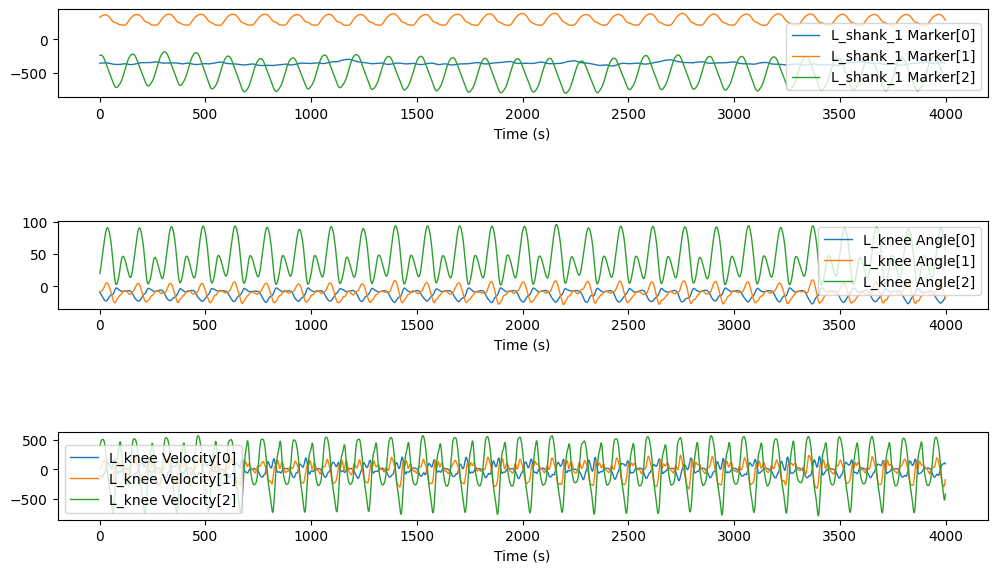
\includegraphics[width=\textwidth]{images/ex_marker_angle_vel_ts.png}
        \caption{Example time series from a single session showing the first left shank marker, left knee angle, and left knee angular velocity across the three axes: [0] X, [1] Y, [2] Z.}
        \label{fig:data-ext-marker-velo-angle-ts}
    \end{minipage}
\end{figure}

\begin{figure}[ht]
    \centering
    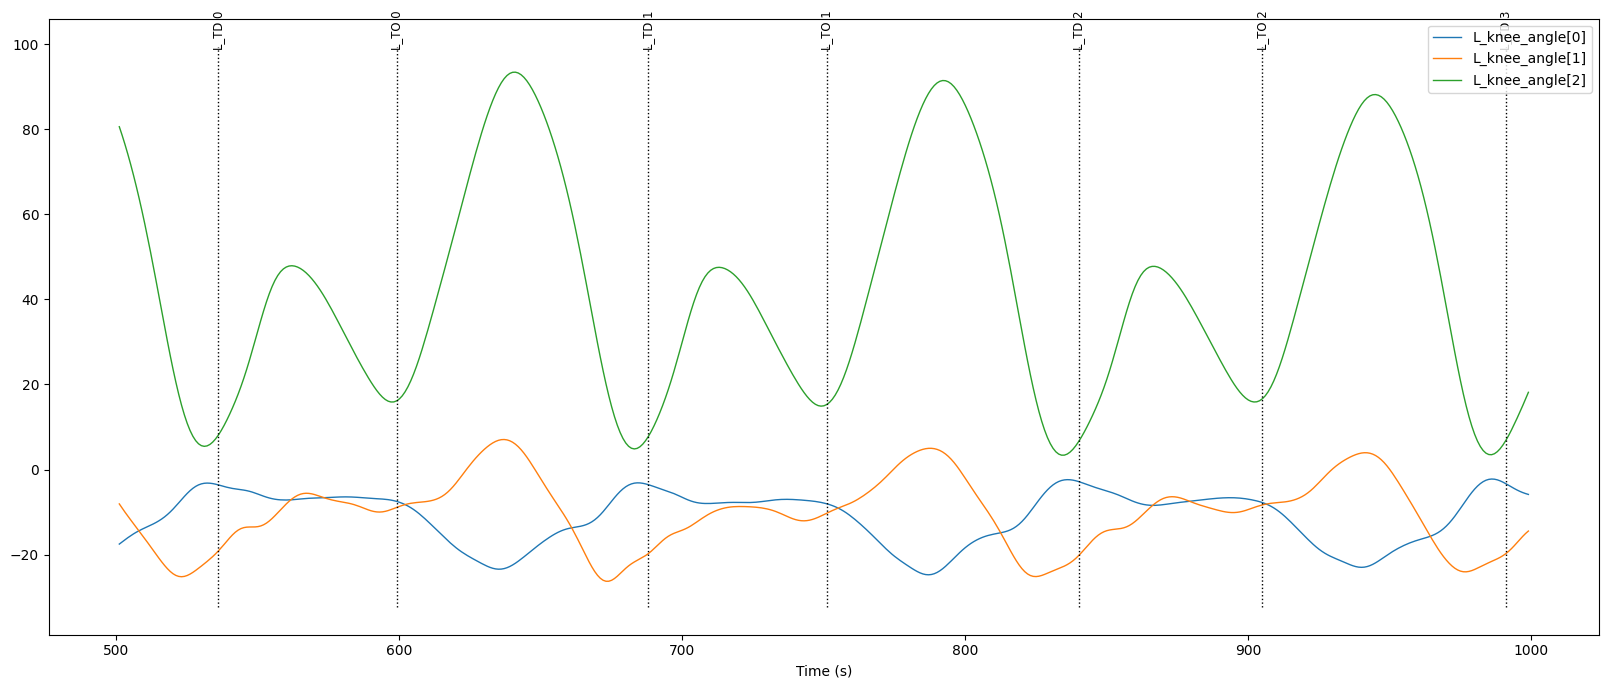
\includegraphics[width=0.5\columnwidth]{images/ex_l_knee_angle_events.png}
    \caption{Frames 500--1000 of the left knee angle (three axes: [0] X, [1] Y, [2] Z), annotated with touchdown (\(L\_TD\)) and toe-off (\(L\_TO\)) events.}
    \label{fig:data-ext-l-knee-angle-events}
\end{figure}


\section{Exploratory Data Analysis (EDA)}\label{sec:method-eda}
As discussed on the previous section, we have two main types of data available:

\begin{itemize}
    \item \textbf{Tabular datasets}
    \begin{itemize}
        \item Session metadata, a set of anthropometric and demographic variables.
        \item Descriptive variables, a engineered set of biomechanical variables derived from the joint angles and angular velocities.
    \end{itemize}
    \item \textbf{Time-series datasets}
    \begin{itemize}
        \item Joint angles derived from the marker data.
        \item Joint angular velocities derived from the marker data.
    \end{itemize}
\end{itemize}

Given the difference in structure of both groups of datasets we need to apply different techniques and methods when working with them. Below we will discuss each of them separately.

\subsection{Tabular dataset}\label{subsec:method-tabular-dataset}
The tabular datasets contain a row for each of the 1813 recordings of running sessions. There are 1394 distinct runners within those sessions, with 207 of them having more than 1 session recorded.

\paragraph{Categorical Variable Cleaning and Encoding}
The values of nominal categorical variables with less than 100 categories have been mapped to a code that is easier to work with(no spaces, no special characters and restricted length), and we have consolidated categories that refer to the same code but were written slightly differently (i.e. meniscal tear-lateral and meniscal tear lateral).

For nominal categorical variables with more than 100 categories that are likely a free text input for the subjects like \texttt{Activities}, we Convert to lowercase, remove leading and trailing spaces, replace non-standard separators with comma, replace multiple spaces with single space, replace multiple commas with single comma.

For ordinal categorical values, we have introduced both a code and a numerical representation so that we can choose what to use depending on the task.
Quantitative variables have been left unchanged, standardisation and normalization has been left for a later stage.

All values that do not fall into a defined category or an accepted value for the data-type are considered as missing value and are converted to None. This is saved as "" when saving the dataset to CSV format.

> TODO: Expand each of the points and add visualization if needed.

Key points regarding the distributions of the columns:
\begin{itemize}
    \item The male/female distribution is balanced (exact percentage to be reported), with few empty values.
    \item The \texttt{DominantLeg} variable is skewed towards the right leg, as expected; there are few ambidextrous cases.
    \item The distributions of \texttt{SpecInjury} and \texttt{InjDefn} are noteworthy and should be reported.
    \item The "Level" variable (recreational vs. competitive) is skewed towards recreational runners.
    \item There is little longitudinal data: only 30 sessions (2.1\%) are at least one month apart.
\end{itemize}

\paragraph{Data Quality and Outlier detection}
During inspection of the dataset, several inconsistencies were identified. In some cases, the level of athletic activity (\texttt{Level}), the reported dominant leg (\texttt{DominantLeg}), and the injury descriptors (\texttt{SpecInjury} and \texttt{InjDefn}) changed across sessions for the same subject. These cases were considered plausible and interpreted as part of the natural variability of the dataset. No indication was found in the source paper that such cases should be regarded as data quality issues, and they were therefore left unchanged.

One case was found in which the reported age differed by ten years between two sessions, which exceeds the duration of the study. To investigate, the entire dataset was checked for inconsistencies between reported age and the time difference between sessions. Two problematic cases were identified:
\begin{itemize}
    \item Subject 100234 was recorded as 40 years old in the first session and 43 years old one year later. In this case, the age in the second session was corrected to 41.
    \item Subject 200375 was recorded as a 27-year-old female in one session and as a 50-year-old male in the next. This inconsistency suggests that the sessions belong to different individuals. A new synthetic subject identifier (300375) was therefore created, and the second session was reassigned to this new subject. The total number of sessions remained unchanged, but the number of unique subjects increased by one.
\end{itemize}

Additional inconsistencies were found in the injury variables. In many sessions, \texttt{SpecInjury} was empty while \texttt{SpecInjury2} contained information. These cases were treated as input errors: when \texttt{SpecInjury} was missing and \texttt{SpecInjury2} was populated, the value of \texttt{SpecInjury2} was taken as the primary injury. A subject was assumed to have no primary injury in a session only if both fields were empty.

All columns in the metadata were inspected for implausible values. Table \ref{tab:met-outlier-range} summarises the range thresholds used for outlier detection. Values outside of these ranges were considered unrealistic and replaced with \texttt{None}. For example, ages of 255~years, heights of 999~cm, weights of 1564~kg, injury durations of 30,000~days (82~years), and years running of 999 were identified as outliers and removed. These extreme values were detected visually using box plots and validated against plausible ranges for human adults.


%TODO: Try to get it to show together with the text
\begin{table}[htbp]
    \centering
    \caption[Outlier detection range for tabular data]{Summary of outlier detection ranges for key variables.\label{tab:met-outlier-range}}
    \begin{tabular}{lcc}
        \hline
        \textbf{Variable} & \textbf{Min} & \textbf{Max} \\
        \hline
        Age & 18.0 & 73.0 \\
        Height (cm) & 120.0 & 196.5 \\
        Weight (kg) & 42.5 & 176.0 \\
        Injury duration (days) & 0.0 & 176.0 \\
        Years running & 0.0 & 54.0 \\
        \hline
    \end{tabular}
\end{table}


\paragraph{Merging metadata and biomechanical variables}
A surrogate key \texttt{id} was introduced to uniquely identify each sample across datasets, where one sample corresponds to a session. The surrogate key was defined as the concatenation of the subject identifier and the session filename in uppercase (e.g., \texttt{100001\_20110531T161051}). This column was then used as the join key to merge the metadata and biomechanical variables.
% TODO: List all variables available? Maybe better on a Apendinx?

\paragraph{Missing values}
Table\ref{tab:met-missing-values} presents the ten variables with the highest proportion of missing values after standardisation, data cleaning, and outlier detection. We decided to keep all discrete variables and \texttt{age}, \texttt{Height}, \texttt{Weight}, \texttt{Gender} and \texttt{DominantLeg}.

For numeric variables, the maximum proportion of missing values was 0.7\%. However, dropping all rows with at least one missing value would have removed more than twice as many samples. To preserve data, missing values in numeric variables were therefore imputed with the median. The median was chosen because normality could not be assumed for all variables and several distributions were skewed. Under such conditions, the median is more robust than the mean.

For categorical variables, missing values were replaced with the label \texttt{unknown} to allow easy identification of imputed categories.

\begin{table}[htbp]
    \centering
    \caption[Top 10 metadata variable with most missing values]{Top 10 Variable with the highest percentage of missing values after cleaning.\label{tab:met-missing-values}}
    \begin{tabular}{lc}
        \hline
        \textbf{Column} & \textbf{Missing (\%)} \\
        \hline
        YrPR & 77.16 \\
        RaceTimeSecs & 75.95 \\
        NumRaces & 72.91 \\
        RaceTimeHrs & 70.04 \\
        RaceTimeMins & 62.05 \\
        YrsRunning & 31.16 \\
        DominantLeg & 19.46 \\
        RaceDistance & 18.64 \\
        Activities & 17.42 \\
        Level & 14.83 \\
        \hline
    \end{tabular}
\end{table}


\paragraph{Definition of Injury status}
Seven columns contain injury data: primary injury data (\texttt{SpecInjury}, \texttt{InjJoint}, \texttt{InjSide}), secondary injury data (\texttt{SpecInjury2}, \texttt{InjJoint2}, \texttt{InjSide2}), and injury severity (\texttt{InjDefn}), and while primary and secondary injury data is consistent within each group, they are not consistent with injury severity. In total, 9\% of the dataset wither was diagnosed with no injury but the runner reported, at least, that they were "continuing to train in pain" or was diagnosed with an injury but reported \texttt{"no injury"} in the severity score.

The source paper does not precise clearly what logic did they use for a subject to be counted as uninjured, but we have decided to use the information coming from \texttt{SpecInjury} and \texttt{SpecInjury2} because it is medically diagnosed by a medical practitioner. So if any of these two variables has a value other than \texttt{"no\_injury"}, we will flag the runner as injured during the session. The distribution of injured vs uninjured sessions is 63.5\% to 36.5\%.


\paragraph{Variable standardisation for training}\label{para:met-var-standarisation}
To prepare the variables for training, numerical values were standardised using the Z-score $Z = (X - \mu) / \sigma$. This procedure centres the data around a mean of 0 and scales it to a standard deviation of 1. Standardisation reduces bias when working with variables of different magnitudes and is required for models such as Logistic Regression and Support Vector Machine (SVM).

Categorical variables were converted into sparse one-hot encoded arrays, where each category value is represented as a separate column and encoded with a 1 or 0 to indicate its presence. To mitigate perfect collinearity, where one variable can be predicted exactly from another, reducing the reliability of coefficient estimates and hindering interpretability, the column corresponding to the value \texttt{unknown} was dropped for each categorical variable.

It is important to note that any normalisation and imputed values where obtained from the training set only. This ensures that no data leakage from the test and validation set is passed down to the model.

\paragraph{Statistical assessment of predictor-target associations}
t-distributed Stochastic Neighbor Embedding (t-SNE) is a non-linear dimensionality reduction technique that projects high-dimensional data into a low-dimensional space while preserving local neighbourhood relationships \citep{JMLR:v9:vandermaaten08a}. In this project, t-SNE was applied as an exploratory tool to assess whether natural clustering exists in the data. Seven plots were generated with different values of the hyperparameter \texttt{perplexity}, and the plot that best reflected the data structure was chosen. The range of perplexity values proposed in \citet{JMLR:v9:vandermaaten08a} as typical was used.

\begin{figure}[ht]
    \centering
    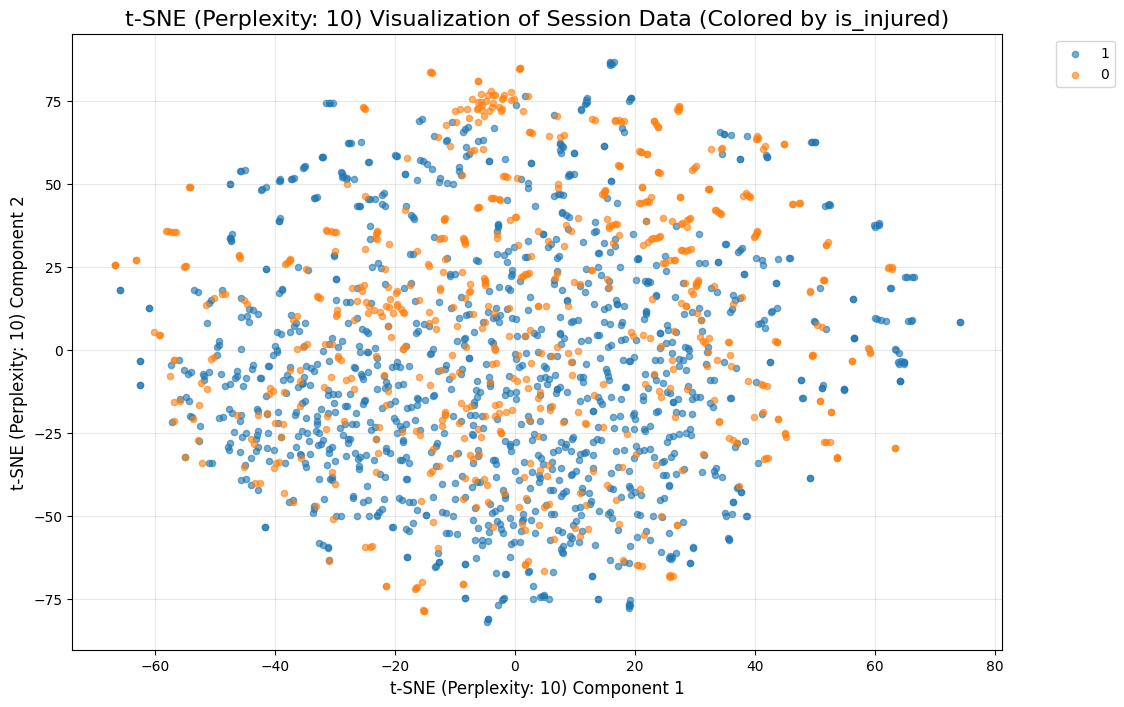
\includegraphics[width=0.5\columnwidth]{images/t-sne-p10-scatter-is_injured.png}
    \caption[2D t-SNE plot with perplexity 10]{2D t-SNE plot with perplexity 10. Injured samples appear in blue and uninjured samples in orange.\label{fig:met-tsne-injured}}
\end{figure}

Figure~\ref{fig:met-tsne-injured} shows the 2D t-SNE projection of the cleaned dataset. The embedding suggests that no strong natural groupings exist, as injured and uninjured samples overlap across most of the plot. A small cluster of uninjured samples is visible in the upper-central region, but the distance to neighbouring points is limited. This indicates that even the most distinct subgroup is not well separated and that class separation is more complex due to high similarity between classes. It should also be noted that the figure only displays the first two t-SNE components. Additional separation may exist in higher-dimensional representations.

The plot also highlights differences in the relative density of the two classes: injured samples appear more frequently in the lower-left region, whereas uninjured samples are more common in the upper-centre. A separating line could be drawn such that more than 50\% of the uninjured samples fall on one side, suggesting that a simple linear classifier trained on the t-SNE components would perform slightly better than random chance. This indicates that some degree of class separation is present, although it remains weak.

To complement the visual inspection, statistical tests were performed to quantify the relationship between predictors and the target variable. Mutual information (MI) was computed for all variables, Pearson's correlation coefficient was calculated for numerical predictors, and independent-sample t-tests were applied to compare distributions of injured and uninjured groups. For categorical variables, Chi-squared tests were performed. Table~\ref{tab:met-top-vars-stat-test} shows the top-scoring predictors under each metric.

\begin{table}[htbp]
    \centering
    \caption{Top predictors of injury status across statistical tests. \label{tab:met-top-vars-stat-test}}
    \begin{tabular}{lll}
        \hline
        \textbf{Metric} & \textbf{Predictor} & \textbf{Score} \\
        \hline
        \multicolumn{3}{l}{\textit{Top 5 by Mutual Information}} \\
        & weight & 0.069027 \\
        & age & 0.045877 \\
        & height & 0.043159 \\
        & dom\_leg\_foot\_ang\_at\_hs & 0.021200 \\
        & dom\_leg\_diff\_knee\_abd\_peak\_angle & 0.021124 \\
        \hline
        \multicolumn{3}{l}{\textit{Top 5 by absolute correlation with is\_injured}} \\
        & dom\_leg\_stance\_time & Pearson $r$ = 0.228451, $p$ = $6.78 \times 10^{-23}$ \\
        & dom\_leg\_stride\_length & Pearson $r$ = -0.166545, $p$ = $9.58 \times 10^{-13}$ \\
        & dom\_leg\_ankle\_eve\_peak\_vel & Pearson $r$ = 0.149308, $p$ = $1.67 \times 10^{-10}$ \\
        & dom\_leg\_hip\_ext\_peak\_angle & Pearson $r$ = 0.139237, $p$ = $2.62 \times 10^{-9}$ \\
        & dom\_leg\_pelvic\_drop\_peak\_vel & Pearson $r$ = -0.133314, $p$ = $1.21 \times 10^{-8}$ \\
        \hline
        \multicolumn{3}{l}{\textit{Top 5 by t-test p-value}} \\
        & dom\_leg\_stance\_time & $6.78 \times 10^{-23}$ \\
        & dom\_leg\_stride\_length & $9.58 \times 10^{-13}$ \\
        & dom\_leg\_ankle\_eve\_peak\_vel & $1.67 \times 10^{-10}$ \\
        & dom\_leg\_hip\_ext\_peak\_angle & $2.62 \times 10^{-9}$ \\
        & dom\_leg\_pelvic\_drop\_peak\_vel & $1.21 \times 10^{-8}$ \\
        \hline
        \multicolumn{3}{l}{\textit{Top 1 by Chi$^2$ p-value}} \\
        & gender & 0.193481 \\
        \hline
    \end{tabular}
\end{table}

In summary, the correlation and t-test results indicate that several predictors show statistically significant differences between injured and uninjured populations, although this differences are small. Gender, as expected, was not statistically significant. Interestingly, variables highlighted by MI did not always overlap with those identified by correlation or t-tests, since MI is able to capture non-linear dependencies. However, some of the variables with the highest MI scores (i.e., weight, height) are unlikely to be causal predictors of injury status. This suggests that models focusing heavily on such variables may fail to generalise well and should be taken into consideration when addressing explainability of the models.


% Should I add this? not for now....
% \begin{itemize}
%     \item Compare populations with mann-witney statistical test
% \end{itemize}


\subsection{Time-series dataset}\label{subsec:method-ts-dataset}
The time-series dataset contains the projection of the joint angles and angular velocities of nine joints (left and right foot, ankle, knee, and hip, plus the pelvis) on three axes (X, Y, Z), which have been derived from the 3D marker data of a session. This results in a total of 54 time series per session.

99\% of the sessions were recorded at 200~Hz and lasted up to 60~seconds, which means that each time series contains up to 12,000 data points. This is too large for direct use. In addition, to use this time-series data in machine learning models or for fair comparisions, each time point must represent the same point in the phase of the movement across all sequences. This is not the case in our datasets due to differences in length, sampling frequency, and starting points for each session. Additionally, there is inter subject variability and intra-session variability to be considered \citep{Chau2005}.

Alignment methods exist, such as Dynamic Time Warping \citep{Bringmann2023}, that could be used to mitigate this problem, but the same goal can be achieved with methods far less complex, for example by simply segmenting and normalising the data.

\paragraph{Stance phase segmentation and normalisation}
Following the procedure described in the source paper \citep{Ferber2024} and later replicated with good results in \citep{FuentesJimnez2025}, we discard the swing phase of the movement and, segment each recording by the stance phases, that is the time when the foot is touching the ground. To perform this segmentation, each \gls{channel} was split using the the gait events dataset introduced in \ref{subsec:data-extraction}. The stance phase starts with touchdown (TD) and ends with toe-off (TO).

It should be noted that the stance phases of the right and left sides overlap whenever both feet are in contact with the ground. For this reason, different events were used to segment the two sides. Specifically, the events \texttt{L\_TD} and \texttt{L\_TO} were used for left-side joints, while \texttt{R\_TD} and \texttt{R\_TO} were used for right-side joints.

The pelvis was treated as a special case, since it is not side-specific. For this joint, two groups of segments were created: one aligned with the left stance phase and one aligned with the right stance phase. This segmentation procedure was applied to both angles and angular velocities. Table \ref{tab:met-ts-vars} lists all time-series variables available per session, which add up to 60 in total.

The duration of the stance phase varies even within a session, figure~\ref{fig:met-hist-segments} shows the distribution of segment duration within a session, which ranges from 62 to 67 frames. To be able to compare segments fairly, it is standard practice to normalise biomechanical kinematic data to 101 data points \citep{Crane2010,FuentesJimnez2025}, representing the percentage of the stance phase from 0\% to 100\% inclusive. When normalising the segments, linear interpolation is used.

\begin{figure}[ht]
    \centering
    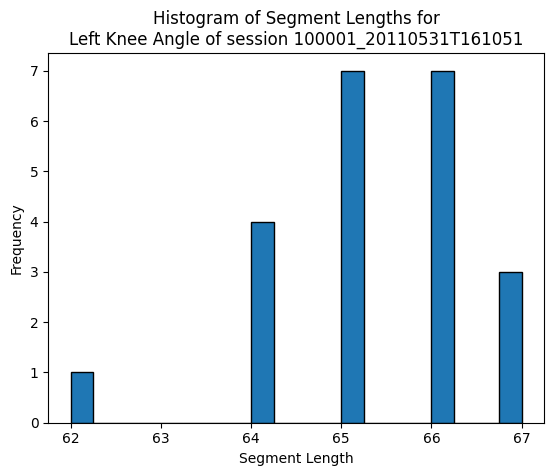
\includegraphics[width=0.5\columnwidth]{images/hist_segment_lengths_L_knee_angle.png}
    \caption[Histogram of Segment Lengths for a session]{Histogram of Segment Lengths for the Left Knee Angle of session 100001\_20110531T161051.\label{fig:met-hist-segments}}
\end{figure}

\subsection{Feature Engineering}\label{subsec:method-feature-engineering}
High collinearity was observed within the tabular dataset, which is expected in the biomechanics domain since the variables we work with are usually describing the same movement or posture (e.g., stance time is inversely proportional to running speed and strongly related to stride length). A correlation matrix confirmed that several variables were highly correlated, and initial variance inflation factor (VIF) values were extremely high.

To reduce redundancy and at the same time generate more informative predictors, new features were engineered based on the symmetry of the lower limbs. For each left-right pair of variables, only the measurement from the dominant leg was retained (i.e. for a right dominant leg runner, pelvis\_peak\_drop\_angle\_left was dropped and pelvis\_peak\_drop\_angle\_right was renamed to dom\_leg\_pelvis\_peak\_drop\_angle). When the dominant leg was not reported or was marked as ambidextrous, the right side was selected by default, as it is the most common case in the dataset.

In addition, to preserve information from the non-dominant side, new **difference variables** were created to capture asymmetries between the two legs. These were defined as:
\begin{equation}
    x_{\mathrm{diff}} = x_{\mathrm{dom}} - x_{\mathrm{nondom}}
\end{equation}
where $x_{\mathrm{dom}}$ is the value for the dominant leg and $x_{\mathrm{nondom}}$ is the value for the non-dominant leg. The new variables were named with the following convention: dom\_leg\_diff\_\$VariableName i.e. dom\_leg\_diff\_step\_width for the difference between step\_width\_right and step\_width\_left.

Interestingly, the step width was found to be symmetrical across all sessions. This variable was computed in \texttt{gait\_steps.m}, and the observed symmetry is likely a result of the estimation process applied to the marker data. The feature \texttt{dom\_leg\_diff\_step\_width} was therefore dropped from the dataset, as it contained only zeros.  

As a result, the biomechanical variable set was reduced from 80 variables (40 per side) to 79 variables: 40 for the dominant side and 39 asymmetry variables.  

The set of biometric and demographic variables was also reduced. Only variables with less than 5\% missing values were retained, which led to the removal of activity and experience-related variables. The variables preserved were \texttt{Age}, \texttt{height}, \texttt{weight}, \texttt{gender}.  

Finally, since \texttt{DominantLeg} was already incorporated into the dataset through the symmetry features, this variable was removed. After feature engineering, the final variable set contained 83 variables: 79 biomechanical and 4 biometric/demographic.

This feature engineering step not only reduced the dimensionality of the predictor set but also introduced meaningful asymmetry measures that may be biomechanically relevant for injury detection. After applying this transformation, VIF values decreased substantially: the number of variables with VIF $< 10$ increased from 10 to 32, and the remaining variables above this threshold showed much lower values than before.

\subsection{Feature Selection}\label{subsec:method-feature-selection}
Two complementary methods were used, one per dataset type: (i) a filter-wrapper approach with Minimum Redundancy-Maximum Relevance (mRMR) to select best performing predictors for the tabular dataset, and (ii) a session-level summarisation of time-series curves to build compact, comparable representations for each joint angle and velocity.

\paragraph{Tabular features: mRMR}
To reduce redundancy while keeping predictive capacity, mRMR \citep{DING2005} was applied to the training set after preprocessing and feature engineering. The goal of mRMR is to maximise feature-target relevance while minimising redundancy among selected features.

\begin{equation}
TODO: EXPLAIN-MRMR-METHOD
\end{equation}

In practice, the MRMR implementation from \texttt{feature\_engine} python package was used with a Random Forest classifier as the relevance model, tuned via 3-fold cross-validation and optimised for ROC-AUC, and Pearson's correlation coefficient was used as redundancy measure.

\begin{figure}[ht]
    \centering
    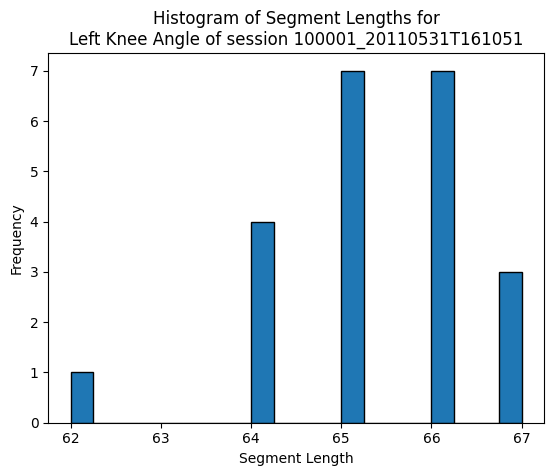
\includegraphics[width=0.5\columnwidth]{images/hist_segment_lengths_L_knee_angle.png}
    \caption[Tabular Features by MRMR relative relevance]{Tabular Features by MRMR relative relevance and, in red, the relevance cut-off value. Featured below that threshold were dropped.\label{fig:met-mrm-feat-sel}}
\end{figure}

All 83 variables were standardised following the steps outlined in paragraph~\ref{para:met-var-standarisation}, which means that all columns were z-score normalised, missing values were replaces with the median of the column, \texttt{gender}, the only categorical column left, was encoded into \texttt{gender\_male} and \texttt{gender\_female}. This elevated the variable count to 84.

All 84 columns were considered by the MRMR algorithm, and the top 40 were selected reducing the dataset by 52\%. Figure \ref{fig:met-mrm-feat-sel} shows the relative relevance of each feature and the cut-off value used.

Later in this document, in subsection \ref{subsec:method-data-config}, the different dataset configuration are detailed and discussed.

\paragraph{Time-series curves: session-level summarisation}
\citet{Chau2005} acknowledges that inter-sample variation of the gait cycle is common across a sample of single-gait cycles and highlights that poor summarisation when combining multiple cycles into one can lead to the cancellation of critical shape characteristics and landmarks. Moreover it proposes the Curve Registration technique \citep{Ramsay1998} as an effective way to maintain key curve features after summarisation.

In \citet{Ramsay1998} curve registration is described as "the process of aligning curves by identifying the timing of certain salient features in the curves", or to put it in other words, to align the time axis of one or more time-series such that each data-point $x_t$ on time $t$ represents the same landmark as a reference curve. Multiple registration techniques exist. In \citet{Chau2005} and iterative registration process is discussed based on global registration, and Dynamic Time Warping (DTW). The iterative process is described as: "The basic principle is then to repeatedly align a set of sample functions to an iteratively estimated mean function. The agreement between a sample function and the mean function can be measured by a sum-of-squared error criterion. The goal of registration is to find a set of temporal shift functions such that the evaluation of each sample function at the transformed temporal values minimizes the sum-of-squared error criterion."

In this project, we have implemented an iterative Curve Registration with DTW. We used the \texttt{dtw} python library \citet{Giorgino2009} for the estimation of the best alignment between two curves. The pseudo code for the algorithm can be found \ref{alg:curve-registration-dtw}:

\begin{algorithm}
\caption{Iterative DTW-based Curve Registration}
\begin{algorithmic}[1]
\Require curves $\in \mathbb{R}^{N \times T}$, max\_iter $\in \mathbb{N}$, tol $> 0$, step\_pattern
\Ensure representative $\in \mathbb{R}^T$
\State registered\_curves $\gets$ curves
\For{$\text{iter} \gets 0$ to $\text{max\_iter} - 1$}
    \State template $\gets \mathrm{Mean}(\text{registered\_curves}, \text{axis}=0)$ \Comment{$\in \mathbb{R}^{T}$}
    \State new\_registered $\gets$ empty list
    \ForAll{curve $\in$ curves}
        \State alignment $\gets \mathrm{DTW}(\text{curve}, \text{template})$
        \State $\text{path\_x} \gets \text{alignment.index1}$ \Comment{Indices in \textbf{curve}...}
        \State $\text{path\_y} \gets \text{alignment.index2}$ \Comment{... mapped to indices in \textbf{template}.}
        \State aligned $\gets \mathbf{0}_T$; counts $\gets \mathbf{0}_T$
        \ForAll{$(i, j)$ in zip(path\_x, path\_y)}
            \State aligned[$j$] $\gets$ aligned[$j$] $+$ curve[$i$] \Comment{Accumulate aligned \textbf{curve} values.}
            \State counts[$j$] $\gets$ counts[$j$] $+ 1$
        \EndFor
        \For{$j \gets 0$ to $T-1$}
            \If{counts[$j$] $>$ 0}
                \State aligned[$j$] $\gets$ aligned[$j$] / counts[$j$] \Comment{Average aligned points.}
            \Else
                \State aligned[$j$] $\gets 0$
            \EndIf
        \EndFor
        \State append(new\_registered, aligned)
    \EndFor
    \State prev $\gets$ registered\_curves
    \State registered\_curves $\gets \mathrm{StackRows}(\text{new\_registered})$ \Comment{$\in \mathbb{R}^{N \times T}$}
    \If{$\text{iter} > 0$}
        \State change $\gets \mathrm{Mean}(|\text{registered\_curves} - \text{prev}|)$
        \If{change $<$ tol}
            \State \textbf{break}
        \EndIf
    \EndIf
\EndFor
\State \Return $\mathrm{Mean}(\text{registered\_curves}, \text{axis}=0)$
\end{algorithmic}
\end{algorithm}

The resulting representative curve provides a compact description of a runner's movement pattern while preserving temporal structure, and it can be used both for visual inspection and as input features for further analysis.

$TODO ADD FIGURE of Curve registration with different algorithms.$

Several algorithms are available for DTW estimation, each producing markedly different results. After visual inspection, the Rabiner-Juang step pattern \citep{Rabiner1993}, configured with family~$VI$ and subtype~$C$\footnote{A detailed description of available step patterns in DTW can be found in the documentation of the R version of the library: \url{https://search.r-project.org/CRAN/refmans/dtw/html/stepPattern.html}.}, was selected as the most stable option.

However, the iterative nature of the algorithm resulted in very poor processing performance. Executing DTW across the full set of curves required more than 30~days of computation on the available resources, even when parallelised across 8~cores. With this computational cost the approach is impractical within the resource constraints of the project. As an alternative, a simple mean curve was computed as a faster approximation. Although less precise, this approach produced results in line with project requirements. With additional time and computational resources, the DTW procedure could potentially be reformulated into a matrix-based optimisation problem, which would improve scalability and efficiency.


$TODO ADD FIGURE of Curve registration compared with mean.$

Overall, this two-pronged strategy reduced dimensionality and redundancy in the tabular space while producing a single time-series representations for each feature in a session.


\section{Modelling}\label{sec:method-models}

\subsection{Data Partitioning and Evaluation Protocol}\label{subsec:method-eval-proto}
In order to ensure a robust evaluation of the models and to avoid data leakage between training and testing phases, a group-aware splitting strategy was adopted at the subject level. This guarantees that all sessions from the same subject appear exclusively in one partition (train, validation, or test).

This decision wsa motivated by the risk of data leakage due to a model learning specificities of a subject that can be used to inflate the validation and test score. By ensuring that all sessions of a subject fall on the same partition, overfitting is reduced.

\paragraph{Train, validation, and test sets}
The dataset was divided into three partitions:
\begin{itemize}
    \item \textbf{Training set}: used primarily for fitting the models.
    \item \textbf{Validation set}: used primarily for optimal threshold detection and performance monitoring in deep learning models.
    \item \textbf{Test set}: used exclusively for model evaluation. As an unbiased estimate of model performance.
\end{itemize}

The training set was used to fit the models. For the tabular models, part of the training set was used  within a cross-validation scheme during grid search in order to evaluate the performance of different hyperparameter configurations.

The validation set was used to determine the optimal decision threshold for classification both for tabular and deep learning models. This ensured that the threshold calibration was unbiased.

For the deep learning models, the training set was used exclusively to optimise model weights, while the validation set was used exclusively to monitor model performance during training. The validation loss guided early stopping and was used for model checkpointing.

The final split proportions were set to \texttt{70\%} for training, \texttt{10\%} for validation, and \texttt{20\%} for testing for the tabular models, and \texttt{60\%} for training, \texttt{20\%} for validation, and \texttt{20\%} for testing.

A bigger validation set ratio was choosen for the deep learning models because of the role it plays in that pipeline. Since it is used to monitor performance, we needed to make sure that the validation had enough samples to represent the population faithfully. On the tabular model pipeline, the validatioin set is only used to estimate the optimal threshold, something that can be done with less samples.

The splits of every partiion were stratified by injury status to preserve the class distribution across partitions. Having a group-aware restriction makes the stratification task very hard. In this project we did a best effort to keep the class balance equal accross partitions. Table \ref{tab:met-data-splits} summarises the actual proportions and class distribution per partition and preprocessing pipeline.


\begin{table}[htbp]
    \centering
    \caption[Train-Test-Validation Split and Class Distribution]{Summary of train, validation, and test splits with class distributions for tabular and deep learning model pipelines.}
    \label{tab:met-data-splits}
    \begin{tabular}{llcccc}
    \hline
    \textbf{Pipeline} & \textbf{Split} & \textbf{Samples} & \textbf{Proportion (\%)} & \textbf{Injured (\%)} & \textbf{Uninjured (\%)} \\
    \hline
    \multirow{3}{*}{Tabular}
      & Train & 1254 & 69.2 & 64.0 & 36.0 \\
      & Validation & 192 & 10.6 & 64.6 & 35.4 \\
      & Test & 367 & 20.2 & 61.0 & 39.0 \\
    \hline
    \multirow{3}{*}{Deep Learning}
      & Train & 1068 & 58.9 & 63.8 & 36.2 \\
      & Validation & 378 & 20.8 & 65.1 & 34.9 \\
      & Test & 367 & 20.2 & 61.0 & 39.0 \\
    \hline
    \end{tabular}
\end{table}


\paragraph{Cross-validation within training in the tabular pipeline}
During hyperparameter tuning in the tabular model pipeline, $k$-fold cross-validation was used with splits taken fro the training set to improve the reliability of model evaluation and to mitigate variance due to partitioning. Specifically, \texttt{k=5} folds were used. Splits were group-aware and stratified by the injury status label like teh training, test and validation set to prevent data leakage.

\paragraph{Evaluation protocol}
The Area Under the Receiver Operating Characteristic curve (\texttt{AUC ROC}) was used as the primary evaluation metric during hyperparameter tuning and model selection. This metric represents the area under the curve obtained by plotting the True Positive Rate (TPR) against the False Positive Rate (FPR) across all possible thresholds. Formally:

\begin{equation}
    \mathrm{TPR}(t)=\frac{\mathrm{TP}(t)}{\mathrm{TP}(t)+\mathrm{FN}(t)},\quad
    \mathrm{FPR}(t)=\frac{\mathrm{FP}(t)}{\mathrm{FP}(t)+\mathrm{TN}(t)},
\end{equation}

\begin{equation}
    \mathrm{AUC}_{\mathrm{ROC}}
    = \sum_{i=1}^{m-1} \big(\mathrm{FPR}_{i+1}-\mathrm{FPR}_{i}\big)\,
    \frac{\mathrm{TPR}_{i+1}+\mathrm{TPR}_{i}}{2}.
\end{equation}

Here $TP(t)$, $TN(t)$, $FP(t)$, and $FN(t)$ represent the number of true positives, true negatives, false positives, and false negatives at a threshold $t$, respectively. $\mathrm{AUC}_{\mathrm{ROC}}$ was approximated using the trapezoidal rule on $m$ thresholds, typically corresponding to the unique scores returned by the model. Since \texttt{AUC ROC} is insensitive to class prevalence, it is suitable for comparing model performance across the slightly different class distributions that result from group-aware splits.

The Area Under the Precision-Recall curve (\texttt{AUC PR}) and the macro-averaged F1-score (\texttt{F1-Macro}) were used as secondary metrics. Precision and recall are defined as:

\begin{equation}
    \mathrm{Prec}(t)=\frac{\mathrm{TP}(t)}{\mathrm{TP}(t)+\mathrm{FP}(t)},\quad
    \mathrm{Rec}(t)=\frac{\mathrm{TP}(t)}{\mathrm{TP}(t)+\mathrm{FN}(t)}.
\end{equation}

\begin{equation}
    \mathrm{AUC}_{\mathrm{PR}}
    = \sum_{i=1}^{m-1} \big(\mathrm{Rec}_{i+1}-\mathrm{Rec}_i\big)\,\frac{\mathrm{Prec}_{i+1}+\mathrm{Prec}_i}{2}.
\end{equation}

\begin{equation}
    \mathrm{F1}=\frac{2 * TP}{2 * TP + FP + FN}
\end{equation}

\begin{equation}
    \mathrm{F1}_{\mathrm{macro}}=\frac{1}{K}\sum_{k=1}^{K}\mathrm{F1}_k.
\end{equation}

In these equations, $\mathrm{Prec}(t)$ and $\mathrm{Rec}(t)$ denote precision and recall at threshold $t$, $\mathrm{AUC}_{\mathrm{PR}}$ is computed with the trapezoidal rule on $m$ thresholds, and $K$ is the number of classes (two in this case: injured and uninjured). Unlike \texttt{AUC ROC}, both \texttt{AUC PR} and \texttt{F1-Macro} are sensitive to class prevalence. Therefore, they are not directly comparable across different pipelines (e.g., tabular versus deep learning), but they provide useful complementary insight when comparing runs of the same model or models within the same pipeline.

Probabilistic classifiers such as Logistic Regression, Random Forest, and XGBoost, and calibrated SVMs output probabilities in the range $[0,1]$, where 1 indicates complete confidence that a sample belongs to the positive class. A default threshold of 0.5 is often used, but the optimal value depends on the metric of interest. In clinical contexts, thresholds are frequently set to minimise False Negatives.In this project, the objective was not clinical deployment but balanced model comparison. Therefore, thresholds were selected to maximise the macro-averaged F1-score (\texttt{F1-Macro}), which computes F1 independently for each class and averages them, penalising models that ignore the minority class. This choice ensured balanced performance across classes and provided a consistent basis for reporting precision, recall, and accuracy.


\paragraph{Model comparison protocol}
The secondary objective of the project is to assess whether any of the deep learning models significantly improves the performance of the best tabular model.
$TODO:-Describe-protocol-to-compare-AUC_ROC$
\citep{Sun2014}
% TODO: Describe how we prove that a model has a statistically siginificant advantage over another.
% See https://ieeexplore.ieee.org/document/6851192
% And: https://github.com/yandexdataschool/roc_comparison?tab=readme-ov-file

\subsection{Logistic Regression Model}\label{subsec:method-log-reg}
Logistic regression is a widely used statistical learning method for modeling the relationship between a binary dependent variable and one or more independent predictors. Unlike linear regression, which assumes a continuous outcome, logistic regression is designed for classification tasks where the target variable is categorical, typically taking values of 0 or 1. The model estimates the probability that a given input belongs to the positive class by applying the logistic function to a linear combination of the predictors. This transformation ensures that predicted probabilities are constrained within the interval $[0, 1]$, making the model interpretable in terms of likelihoods.

Mathematically, the logistic regression model can be expressed as
\begin{equation}
    p(X) = \frac{e^{\beta_0 + \beta_1 X}}{1 + e^{\beta_0 + \beta_1 X}},
\end{equation}
where $\beta_0$ is the intercept and $\beta_1$ is the coefficient associated with predictor $X$. Model parameters are typically estimated through maximum likelihood estimation (MLE), with the objective of maximizing the likelihood of the observed data \citep{James2021Logistic}.

\paragraph{Hyperparameters of Logistic Regression}
Multiple hyperparameters are available that can be used to tweak the performance of the model. In this project we have used:
\begin{itemize}
    \item \textbf{Regularization strength} ($C$): The regularization strength, denoted by the $C$ parameter, which is the inverse of the regularization coefficient $\lambda$.
    \item \textbf{penalty}: The penalty function as \texttt{penalty} parameter, which allows to choose the regularisation function to use: $\ell_{1}$ penalty (Lasso) or $\ell_{2}$ penalty (Ridge)
\end{itemize}

The $\ell_{1}$ penalty (Lasso) enforces sparsity by driving some coefficients exactly to zero, thereby performing feature selection, while the $\ell_{2}$ penalty (Ridge) shrinks coefficients smoothly without eliminating them.

\subsection{Random Forest}\label{subsec:method-rand-forest}
Random forests are ensemble learning methods that builds on top of the decision trees by combining a large number of them in order to improve predictive accuracy and control overfitting \citep{Breiman2001}. Each tree in the ensemble is constructed from a bootstrap sample of the training data, and at each split a random subset of predictors is considered. This strategy reduces correlation among trees and increases the overall robustness of the model. The final prediction is obtained by aggregating the outputs of all trees. Random forests are non-parametric, can model complex non-linear relationships, and naturally provide measures of variable importance (intrinsic explainability).

\paragraph{Hyperparameters of Random Forest}
Several hyperparameters influence the behavior and generalization ability of random forests. In this project, the following were explored:
\begin{itemize}
    \item \textbf{n\_estimators}: The number of trees in the forest. Increasing this value generally improves performance but comes at the cost of higher computational requirements.
    \item \textbf{max\_depth}: The maximum depth of each tree. Limiting tree depth helps control overfitting, while unlimited depth (\texttt{None}) allows trees to fully grow.
    \item \textbf{min\_samples\_split}: the minimum number of samples required to split an internal node. Larger values result in shallower trees and may improve generalization.
    \item \textbf{min\_samples\_leaf}: The minimum number of samples required to be at a leaf node. Increasing this value creates smoother decision boundaries by preventing overly specific leaves.
    \item \textbf{max\_features}: The number of predictors to consider when searching for the best split. Common choices are the square root of the total number of features (\texttt{sqrt}) or the base-2 logarithm (\texttt{log2}), both of which promote diversity among trees.
\end{itemize}

By tuning these hyperparameters, the trade-off between bias and variance can be adjusted to achieve an optimal balance between accuracy, robustness, and interpretability in the classification task.

\subsection{Support Vector Machine (SVM)}\label{subsec:method-svm}

Support Vector Machines (SVMs) are supervised machine learning classifiers that aim to find the optimal hyperplane that maximises the margin between classes \citep{Cortes1995}. The training samples that lie on or within the margin are the \texttt{support vectors}; these points alone determine the decision boundary. Non-linear decision surfaces are obtained via kernel functions, which implicitly map inputs to a higher-dimensional feature space where a linear separation may exist. In practice, SVMs often achieve strong generalisation, particularly in high-dimensional settings and when the underlying boundary is close to linear \citep{chang2011guide}.

Unlike probabilistic models, SVMs do not natively output class probabilities. Instead, probabilities are commonly estimated through \textit{Platt scaling}, which fits a sigmoid function to the decision values of the trained SVM. This calibration step provides probability estimates in the range $[0,1]$, enabling threshold-based decision making and the use of metrics such as AUC.

SVMs offer two main hyperparameters: the kernel function and the regularisation parameter $C$. The kernel function $K(x,z)$ defines the feature mapping that projects the data points into another dimensional space. Typical kernels include the linear kernel $K(x,z)=x \cdot z$, the polynomial kernel $K(x,z)=(x \cdot z + c)^d$, and the radial basis function (RBF) kernel $K(x,z)=\exp\!\big(-\gamma \lVert x-z\rVert^2\big)$.\paragraph{Hyperparameters of SVMs} The main hyperparameters are:

\begin{itemize}
    \item \textbf{Kernel function} ($K$): Defines the feature mapping to a higher-dimensional space. Typical choices are the linear kernel $K(x,z)=x \cdot z$, the polynomial kernel $K(x,z)=(x \cdot z + c)^d$, and the radial basis function (RBF) kernel $K(x,z)=\exp\!\big(-\gamma \lVert x-z\rVert^2\big)$. Kernel choice controls model flexibility and allows SVMs to tackle non-linear problems.
    \item \textbf{Regularisation parameter} ($C$): Controls the trade-off between maximising the margin and minimising training errors. Smaller $C$ imposes stronger regularisation (wider margins, higher bias), whereas larger $C$ penalises violations more heavily (narrower margins, lower bias but higher variance). 
    \item \textbf{Kernel scale} ($\gamma$): Relevant for non-linear kernels (e.g., RBF and polynomial). Larger $\gamma$ produces more local and complex decision boundaries, whereas smaller $\gamma$ enforces smoother, more global boundaries.
\end{itemize}

By tuning these hyperparameters, the bias-variance profile can be adjusted to balance accuracy and robustness in the classification task.


\subsection{Extreme Gradient Boosting (XGBoost)}\label{subsec:method-xgboost}
Extreme Gradient Boosting (XGBoost) is an ensemble method based on gradient-boosted decision trees that builds a sequence of shallow trees, each one correcting the residual errors of the preceding ensemble \citep{Chen2016XGBoost}. Trees are added in an additive manner (boosting) and are fit by following the gradient of a differentiable loss. Compared with generic gradient boosting, XGBoost introduces explicit regularization on tree complexity, shrinkage (learning rate), and row/column subsampling, which together reduce variance and improve generalization. The method is efficient on tabular data, captures non-linear interactions, and offers robust handling of class imbalance and missing values via built-in mechanisms.

\paragraph{Hyperparameters of XGBoost}
In this project, the following hyperparameters were explored:
\begin{itemize}
    \item \textbf{n\_estimators}: Number of trees. More trees increase capacity and typically require a lower learning rate.
    \item \textbf{max\_depth}: Maximum tree depth. Shallower trees control overfitting and often perform well on noisy biomechanical features.
    \item \textbf{learning\_rate}: Shrinkage applied to each tree's contribution; smaller values generally improve generalization at the cost of more trees.
    \item \textbf{subsample}: Fraction of training instances sampled per tree. Row subsampling lowers variance and decorrelates trees.
    \item \textbf{colsample\_bytree}: Fraction of predictors sampled when growing each tree. Column subsampling mitigates collinearity and encourages diversity.
    \item \textbf{gamma}: Minimum loss reduction required to make a split. Larger values prune weak splits and yield simpler trees.
    \item \textbf{scale\_pos\_weight}: Gradient/Hessian scaling for the minority class to address class imbalance (common heuristic: $N_{\text{neg}}/N_{\text{pos}}$).
    \item \textbf{max\_delta\_step}: Cap on the per-tree weight update that stabilizes logistic boosting under severe imbalance or separation.
\end{itemize}
By tuning these hyperparameters, the bias--variance trade-off was controlled through depth, shrinkage, and subsampling, while class imbalance was directly handled via \texttt{scale\_pos\_weight}, leading to a robust classifier for the injury-detection task.

\subsection{Unilateral BiLSTM}\label{subsec:method-unilat-bilstm}
Explain inversion of X and Y axis.
% LSTM V1:
% Layer 0 - Input:
% Each trial (Session) is a tensor of shape (101, 48) Maybe 54 if we include hip.
% So input is (Batch, 101, 48)

% Layer 1 - Normalization:
% Put all 48 channels on a comparable scale so LSTM does not waste capacity in offsets/units.
% Important so that channels do not dominate just because of the units. Makes the model focus on the shapes and dynamics.
% Normalize with the Z-Score per channel.
% Optionally, remove the trial mean


% Layer 2 - First Temporal Encode:
% BiLSTM (64 units, return_sequences=True)
% Since each trial goes from TD to TO, that means that the time is not circular.
% (If circular, add 2 channels: Sin an Cos)

% Since there is a temporal component, we want to make this explicit to the model to that it can use it in the decision gates instead of having to derive it from other variables.
% Our data corresponds to the stance face only, this means that it is not cyclic, it has a hard start and end., For this scenario, a linear phase hint is a good idea.
% We add one extra channel:


% T = 101
% T = 0, 1, …, 100.
% Pt = t / (T -1) = 0, 0.01, 0.02, …, 0.99, 1
% P(0) = 0
% P(50) = 0.5
% P(100) = 1

% But wait, in our dataset our left and right side stance phases start at t=0, but in reality they happen at different moments in time. We are losing inter-limb coordination cues.
% If we would feed the model as it is, we would be introducing a fake synchronisation between both sides.
% We have two options:
% 1- UNilateral Trials -> Treat left and right as two different sessions adding Pt
% 2 - Two tower siamese model -> Train two sequences, one per each side each with it’s own Pt.

% We choose to start with the simplest approach: 1
% If needed we can reuse the architecture of 1 into two later.

% Unilateral Trial:
% Split tensor by left and right from (101, 48) to (101, 24) and then add Pt, so (101, 25)
% When running the model, we should run both sides and combine the probabilities.

% WE NEED TO START THE MODEL AGAIN:

% LSTM V2 - Unilateral:
% Layer 0 - Input:
% Each trial (Session) is a tensor of shape (101, 25)
% Add Pt as 25th feature.

% Layer 1 - Normalization:
% Normalize with the Z-Score per channel.
% Remove the trial set mean (Save it and use the same for validation and Test)

% Layer 2 - Temporal Encoder:
% BiLSTM(64, return_sequence=true). Since it is bidirectional, the feature space increases to 64x2 = 128 Shape (101, 128)
% Add Stabilizers:
% dropout~=0.2 -> Zeros that fraction of activations during training to reduce overfitting -> Explained
% gradient clipping to 1.0

% Layer 3 - Temporal Encoder (Moved to next version)
% BiLSTM(32, return_sequence=true)
% Output (101, 64)
% This second smaller BiLSTM will help refine the patterns from the first while keeping the time resolution
% Note: It can bring overfit since we have a short wave (101 points)
% Recommended only if underfitting is detected:
% Training loss stays hi and plateaus
% Training AUC-PR is low, and prediction probabilities are very close to 0.5 not confident.



% ROT:
% Underfitting = Low Training performance
% Overfitting = High Training but low validation performance

% Layer 4 - Summary:
% GlobalAvgPool1D + GlobalMaxPool1D
% Mean ≈ “how much overall”, Max ≈ “did it spike” → complementary signals.
% example: if an ankle inversion burst at ~10% stance is predictive, max will catch it even if it’s brief; if the whole stance shows elevated knee valgus features, mean will reflect that.


% Layer 5 -  Dense Head: 
% Small regularized
% Dense(32) -> ReLu  (Non linear mixing of pooled features)
% Dropout(0.3) -- Stronger to prevent overfitting
% Optional( LayerNorm/BatchNorm if unstable training)
% Dense(1) -> Sigmoid to get a probability

\subsection{Bilateral BiLSTM}\label{subsec:method-bilat-bilstm}
With and without CNN.
% LSTM V3 - BiLateral:
% Why:
% Here’s why:
% Your label is session-level (injured=1), not leg-specific.
%  The prediction should consider both legs at once. A bilateral head learns how to fuse sides instead of you hand-picking mean/max after the fact.


% Left/right waveforms can be mirrored or even sign-inverted.
%  A symmetry-aware merge (e.g., using [L,R,|L ⁣− ⁣R|,L ⁣⋅ ⁣R] is robust to those inversions and captures asymmetry directly—often the thing that correlates with injury.


% Your trials were rephased per leg (stance only).
%  True cross-leg time alignment is unreliable. Processing each side separately with a shared encoder avoids assuming synchrony; you compare embeddings, not raw timepoints.


% Shared weights = strong inductive bias + fewer params.
%  The same encoder sees left and right, so it learns leg-agnostic gait features and generalizes better with the data you have.


% Built-in invariances you actually want.
%  With the merge features above (and optional sign canonicalization), the model won’t overfit to “left vs right” quirks; it focuses on patterns and differences between legs.


% Better handling of unilateral injuries.
%  If only one side shows pathologic patterns, the bilateral head can up-weight that side (via the merge features) instead of a blunt post-hoc max/mean.


% Cleaner evaluation & fewer plumbing bugs.
%  One model → one probability P(injured)P(\text{injured})P(injured). No more side-specific orientation flips or manual fusion mistakes.


% Diagnostics & interpretability.
%  You get per-side embeddings and an explicit |L-R| channel—handy for analyzing what asymmetries the model used.
\subsection{MC-DCNN}\label{subsec:method-mc-dcnn}
Architure from paper. -> https://drive.google.com/file/d/162jLdyKmxU4A8ynMr8qCI0xFSIsSHDfC/view?usp=sharing


\subsection{Hyperparameter tuning}\label{subsec:method-hyperparam-tuning}
The choice of hyperparameter search method was influenced by the differences in training cost between tabular and deep learning models. Tabular models are comparatively fast to train because they operate on a small set of descriptive variables and do not rely on iterative training across epochs. In contrast, deep learning models are slower because they are trained in epochs on large tensors, in this case the full time-series dataset (60 channels $\times$ 101 values $\times$ 1813 samples). As a result, within the same amount of time, a broader hyperparameter space can be explored for tabular models, making grid search a feasible option. For deep learning models, however, grid search was impractical, and an adaptive search strategy was required.

Grid search is a search strategy in which a set of values is predefined for each hyperparameter, and models are trained and evaluated on all possible combinations of these values. Although computationally expensive, grid search provides a systematic way to explore the hyperparameter space and is effective when the number of parameters and candidate values is limited.

In contrast, Hyperband is a probabilistic, resource-aware optimisation algorithm that adaptively allocates more resources to promising configurations while eliminating poorly performing ones early \citep{Li2018Hyperband}. It combines random sampling of the hyperparameter space with successive halving, in which configurations are trained with increasing budgets (e.g., number of epochs) and only the best-performing candidates are promoted to later stages. This approach enables efficient exploration of wide hyperparameter spaces, which is particularly advantageous for deep learning models where training costs are high.

For the tabular models, grid search was applied to exhaustively evaluate all combinations in the defined hyperparameter space. A five-fold stratified group cross-validation procedure was used within the training data to estimate model performance, thereby preserving the validation set for post-hyperparameter tuning steps such as operating threshold optimisation.

For the deep learning models (MC-DCNN, bilateral LSTM, and unilateral LSTM), hyperparameter search was performed using the Hyperband implementation in \texttt{Keras Tuner} \citep{Li2018Hyperband}. Each candidate configuration was evaluated on a held-out validation split using ROC-AUC as the objective, with early stopping.

\subsection{Dataset configuration}\label{subsec:method-data-config}
We have already discussed the differences in cost between the tabular and deep learning models and how this affected the hyperparameter tuning process. Cost also had an impact on the chosen data configurations. The relative low training cost of tabular models allowed us to try more data configurations with the same resources. For each data configuration, the full hyperparameter tuning process needs to be performed, as even the smallest nuances on the structure of the data can have an impact on the performance of different models and its configuration.

With the reduced training cost, we allowed ourselves to train thee dataset configuraiton:

\begin{itemize}
    \item \textbf{Baseline}: Original set of 80 biomechanical variables plus 4 biometric/demographic. Table~\ref{tab:baseline_features} contains the full list of variables.
    \item \textbf{Dominant Leg based}: Dominant Leg based features as described in the feature engineering subsection\ref{subsec:method-feature-engineering}. Table~\ref{tab:domleg_features} contains the full list of variables.
    \item \textbf{Top 40 Dominant Leg based}: Top 40 features from the Dominant Leg based dataset, selected by mRMR algorith as described in the feature selection subsection\ref{subsec:method-feature-selection}. Table~\ref{tab:top40_features} contains the full list of variables.
\end{itemize}

It is important to note that all data configurations were normalised following the same protocol as described in subsection~\ref{para:met-var-standarisation}. In appendix~\ref{chap:appendix-1-datasets}, tables with the full list of variable and their descriptions can be found.

For deep learning models, only one data configuration was used: The 60 timeseries that combine joint angles and joint angular velocities\ref{subsec:method-ts-dataset}. Each of these \glspl{channel} was normalised following the procedure described in the time-series dataset subsection\ref{subsec:method-ts-dataset} and a representative curve was computed as described in the feature selection subsection\ref{subsec:method-feature-selection}. As a result, 60 channels with a single stance curve normalised to 101 points was used. Table~\ref{tab:met-ts-vars} contains the full list of variables.

This base data configuraiton was then adapted to the architecture of each of the models. For \textbf{Unilateral BiLSTM}, left and right channels where separated and combined into a single 30 channel dataset with double the amount of samples. Before combining them, the X and Y axis of the left side were inverted, otherwise the model would have seen two inverse representations of the same channel that would have made learning more difficult. In addition, a linear phase channel was added to encode the percentage of the stance phase in the data. This artificial channel was build as a linear vector in range $[0, 101]$ with increments of $1$. This resulted in a tensor of $(N, 101, 31)$, where N is the number of sessions (1068 for the trainset).

For \textbf{Bilateral BiLSTM}, left and right channels where also separated and, for each side, a linear phase was also added. The model has two inputs as it processes left and right through a different "tower" and then combines the learned information at the end. This resulted in two input tensors with shape $(N, 101, 31)$ each.

Lastly, for \textbf{Bilateral BiLSTM}, not like for the previous models, the 60 channels were used without splitting or adding a linear phase channel. This resulted in a single input tensor with shape $(N, 101, 60)$.

\paragraph{Hyperparameter Ranges and Best Values}

The following summarizes the hyperparameter search spaces and the best-performing values identified for each model:
%TODO: Add hyperparameter table by model and data configuration.
% \begin{table}[ht]
%     \centering
%     \caption{Hyperparameter search spaces and best values for each model}
%     \begin{tabular}{llll}
%         \toprule
%         \textbf{Model} & \textbf{Hyperparameter} & \textbf{Values} & \textbf{Best} \\
%         \midrule
%         Logistic Regression & $C$ & $10^{[-3,3]}$ & 0.1 \\
%         Logistic Regression & Penalty & \{l1, l2\} & l1 \\
%         Logistic Regression & Solver & \{liblinear\} & liblinear \\
%         \midrule
%         Random Forest & $n_{\text{estimators}}$ & \{100, 200, 300\} & 200 \\
%         Random Forest & max\_depth & \{None, 10, 20\} & None \\
%         Random Forest & min\_samples\_split & \{2, 5, 10, 16\} & 2 \\
%         Random Forest & min\_samples\_leaf & \{2, 5, 8\} & 2 \\
%         Random Forest & max\_features & \{$\sqrt{\phantom{a}}$, $\log_2$\} & $\sqrt{\phantom{a}}$ \\
%         \midrule
%         XGBoost & $n_{\text{estimators}}$ & \{100, 200, 500\} & 500 \\
%         XGBoost & max\_depth & \{3, 6, 9\} & 6 \\
%         XGBoost & learning\_rate & \{0.005, 0.01, 0.1\} & 0.005 \\
%         XGBoost & subsample & \{0.8, 1.0\} & 0.8 \\
%         XGBoost & colsample\_bytree & \{0.8, 1.0\} & 1.0 \\
%         XGBoost & $\gamma$ & \{0, 1, 5\} & 1 \\
%         XGBoost & scale\_pos\_weight & $=$ neg\_pos\_ratio & $\approx 1.78$ \\
%         \midrule
%         Support Vector Machine & $C$ & \{0.1, 1, 10\} & 1 \\
%         Support Vector Machine & Kernel & \{rbf, linear, poly\} & rbf \\
%         Support Vector Machine & $\gamma$ & \{scale, 0.1, 0.01\} & 0.01 \\
%         \midrule
%         Deep CNN & activation\_combo & \{sigmoid\_relu\} & sigmoid\_relu \\
%         Deep CNN & $k_1$ & \{5, 7\} & 5 \\
%         Deep CNN & $f_{1/\text{ch}}$ & \{8, 12\} & 8 \\
%         Deep CNN & pool1 & \{2, 3\} & 2 \\
%         Deep CNN & hidden & \{256, 512, 768\} & 768 \\
%         Deep CNN & fc\_dropout & \{0.0, 0.2, 0.4\} & 0.2 \\
%         Deep CNN & learning\_rate & \{2e$-$4, 4e$-$4, 8e$-$4\} & $4\times10^{-4}$ \\
%         Deep CNN & weight\_decay & \{1e$-$5, 3e$-$5, 1e$-$4\} & $1\times10^{-5}$ \\
%         \midrule
%         Bilateral Two-Tower LSTM & lstm\_units & \{48, 64, 96\} & 48 \\
%         Bilateral Two-Tower LSTM & lstm\_dropout & \{0.15, 0.20, 0.25, 0.30, 0.35\} & 0.15 \\
%         Bilateral Two-Tower LSTM & head\_hidden & \{48, 64, 96\} & 48 \\
%         Bilateral Two-Tower LSTM & head\_units & \{48, 64, 96\} & 96 \\
%         Bilateral Two-Tower LSTM & head\_dropout & \{0.20, 0.25, 0.30, 0.35, 0.40\} & 0.35 \\
%         Bilateral Two-Tower LSTM & learning\_rate & [1e$-$4, 5e$-$4] & $\approx 5\times10^{-4}$ \\
%         Bilateral Two-Tower LSTM & weight\_decay & [1e$-$5, 3e$-$4] & $\approx 1.1\times10^{-5}$ \\
%         Bilateral Two-Tower LSTM & multiscale\_conv & \{True, False\} & False \\
%         Bilateral Two-Tower LSTM & single\_kernel & \{7, 15, 21, 31, 41, 51\} & 51 \\
%         \midrule
%         Unilateral LSTM & head\_units & \{32, 64\} & 64 \\
%         Unilateral LSTM & head\_dropout & \{0.0, 0.2, 0.4\} & 0.2 \\
%         Unilateral LSTM & lstm\_units & \{64, 128\} & 128 \\
%         Unilateral LSTM & lstm\_dropout & \{0.0, 0.2, 0.4\} & 0.0 \\
%         \bottomrule
%     \end{tabular}
% \end{table}

\noindent
See the supplementary material and code repository for the full search grids and additional details.

\section{Explainability}\label{sec:method-explainability}
Explainability maps model behaviour onto domain knowledge so that complex decisions become transparent and human-interpretable. Some algorithms expose parameters or structures that can be interpreted directly (\emph{intrinsic} explainability), but more complex or non-linear models typically require \emph{post-hoc} methods.

\subsection{Intrinsic explainability}\label{subsec:method-intrinsic-explainability}
\paragraph{Tree ensembles (Random Forest, XGBoost).}
For tree-based models, intrinsic importance scores are available from the training process. In Random Forests, importance is computed as the total decrease in node impurity attributable to splits on each feature, aggregated across all trees \citep{Breiman2001}. In this project, \emph{Gini} impurity was used.

Similarly, in gradient-boosted trees such as XGBoost, importance can be defined as \emph{gain} (reduction in training loss from splits using the feature), \emph{weight} (number of times the feature is used in splits), \emph{cover} (average number of samples affected by such splits), among others \citep{chen2016xgboost}. In this project, \emph{gain} was used as the importance metric. As with Random Forests, these quantities are accumulated during training and are readily available for aggregation.

\paragraph{Linear models (logistic regression, linear SVM).}
Linear models can be represented mathematically as $f(X) = \beta_0 + \beta_1X$. Where the weight of vector $\beta_1$ provides an intrinsic attribution to feature importance. The larger the magnitude of the feature component in $\beta$, the stronger the association between feature and the decision boundary. For logistic regression, the model is linear in the logit function, and the coefficients of $\beta$ can be directly interpreted in terms of feature contributions to the log-odds of the positive class. For a linear SVM, the vector of weights defining the separating hyperplane plays an analogous role, with the absolute value of each weight reflecting the relative importance of the corresponding feature. In both cases, $\beta$ can therefore be interpreted as an intrinsic attribution of feature importance.

\paragraph{Reliability of instrinsic metrics.}
It is important to note that impurity-based importances are biased toward features with many unique values (or higher variance) and can be distorted by collinearity. Linear coefficients are sensitive to feature scaling and multicollinearity. For that reason, permutation importance has been used in the project as a post-hoc explainability measure to complement intrinsic metrics.

\subsection{Post-hoc explainability}\label{subsec:method-posthoc-explainability}
This study employed two complementary post-hoc methods: \emph{permutation importance} for global, model-agnostic assessment on tabular models, and \emph{gradient-based saliency maps} for local attributions in deep learning models.

\paragraph{Permutation importance.}  

Permutation importance \citep{Breiman2001,Fisher2018} is a model-agnostic technique that quantifies the contribution of each feature, globally, by measuring the change in model performance when its values are randomly permuted. For a given feature $j$, the values of the $j$-th column in the dataset $D$ are permuted, randomly, $K$ times, breaking the relationship between the feature and the target while preserving the marginal distribution. On each iteration $k$, the model score $s_{k,j}$ is computed on the permuted dataset.  

The importance of feature $j$ is defined as the difference between the baseline score $s$ (obtained on the original dataset) and the average score across the $K$ permutations:  
\[
i_j = s - \frac{1}{K}\sum_{k=1}^{K} s_{k,j}.
\]  

A feature is considered important if shuffling its values leads to a degradation in model performance (i.e., lower score or higher error). Features with little or no impact on the score when permuted are considered less informative.


\paragraph{Gradient-based saliency maps.}  

Gradient-based saliency maps \citep{Selvaraju2017} are local interpretability methods that estimate the importance of each input feature by analysing how sensitive the model's output is to changes in that input. For a given input sample and a model output, the gradient is the partial derivative of the output with respect to the input sample.

The magnitude of this gradient indicates how much the prediction would change in response to small perturbations in feature. Larger magnitudes correspond to higher local importance, as the model's decision is more sensitive to changes in that feature. Unlike permutation importance, which provides a global view, gradient-based saliency maps offer local, instance-specific attributions.


\paragraph{Reliability of post-hoc methods.}
Both gradient-based saliency maps and permutation importance provide valuable insights but are subject to important caveats. Gradient-based saliency maps are highly sensitive to model architecture, input scaling, and local non-linearities, which can produce noisy or unstable attributions and limit their reliability as standalone explanations. In contrast, permutation importance is more stable and model-agnostic, but it can underestimate the relevance of correlated features, since shuffling one predictor may have little effect when others provide overlapping information \citep{molnar2025}.


% \section{Explainability}\label{sec:method-explainability}
% Explainability makes complex AI decisions transparent and trustworthy. Helps improve the field of biomechanincs by treanslating the learnings of the model into some thing interpretable by humands. Some modesl have internal out of the box parameters that can be interpreted easily, but others, usually those that are more complex, don't.

% \subsection{Intrinsic Explainability}\label{subsec:method-intrinsic-explainability}
% \begin{itemize}
%     \item Random Forest, XGboost via feature_importance_
%     \item Linear models: Logistic regression and SVM with Linear Kernel
%     \item Models wihtout intrisic, need to use post-hoc methods.
%     \item What they are and how are they calcualted
%     \item How much can we trust them
% \end{itemize}

% \subsection{Post-hoc Explainability}\label{subsec:method-posthoc-explainability}
% \begin{itemize}
%     \item permutation importance is model-agnostic (it can be used with any predictive model that outputs a score), but gradient-based saliency maps are not, they require a differentiable model.
%     \item But we will only use permutation with tabular models.
%     \item permutation importance for a global view
%     \item Saliency maps for a local view -> Only use on deeplearning models because it 
%     \item SHAPs, Saliency maps, feature permutation?
%     \item What they are and how are they calcualted
%     \item How much can we trust them
% \end{itemize}


% \subsection{Post-hoc Explainability}\label{subsec:method-posthoc-explainability}
% \begin{itemize}
%     \item permutation importance is model-agnostic (it can be used with any predictive model that outputs a score), but gradient-based saliency maps are not, they require a differentiable model.
%     \item But we will only use permutation with tabular models.
%     \item permutation importance for a global view
%     \item Saliency maps for a local view -> Only use on deeplearning models because it 
%     \item SHAPs, Saliency maps, feature permutation?
%     \item What they are and how are they calcualted
%     \item How much can we trust them
% \end{itemize}
